本节使用回退到 ``230 MeV 偏高'' 之前的代码路径后重新生成的两组小网格数据：
\texttt{8x8-7x7-Nx1000} 与 \texttt{12x12-9x9-Nx2000}。
两组均使用 Eq.15 energy model、streaming-full out-of-core、\texttt{energy-chunk=64}、\texttt{lane-chunk=262144} 和 \texttt{idd-stride=1}。
当前二进制对这两个角网格均走 separable real DST kernel 路径。

\[
  (N_x,N_y,N_z,N_g,N_\mu,N_\omega)
  =(1000,8,8,500,7,7)\quad\text{and}\quad(2000,12,12,500,9,9),
  \qquad x_{\max}=40\,\mathrm{cm}.
\]

\subsection*{9.1 时间总结}
\begin{center}
\scriptsize
\resizebox{\textwidth}{!}{%
\begin{tabular}{llrrrrr}
\toprule
grid & case & total s & s/step & energy s & transport s & angle s\\
\midrule
8x8-7x7-Nx1000 & water 100 & 99.253 & 0.09925 & 60.910 & 6.575 & 1.198\\
8x8-7x7-Nx1000 & water 230 & 174.916 & 0.17492 & 111.166 & 10.754 & 1.823\\
8x8-7x7-Nx1000 & bone 100 & 98.985 & 0.09898 & 60.787 & 6.630 & 1.193\\
8x8-7x7-Nx1000 & bone 230 & 177.303 & 0.17730 & 112.056 & 11.279 & 1.896\\
12x12-9x9-Nx2000 & water 100 & 564.906 & 0.28245 & 344.775 & 35.628 & 4.468\\
12x12-9x9-Nx2000 & water 230 & 998.575 & 0.49929 & 632.103 & 55.619 & 7.400\\
12x12-9x9-Nx2000 & bone 100 & 558.692 & 0.27935 & 338.871 & 36.161 & 4.466\\
12x12-9x9-Nx2000 & bone 230 & 993.284 & 0.49664 & 624.786 & 58.465 & 7.372\\
\bottomrule
\end{tabular}%
}
\end{center}

上表中的 \texttt{energy}/\texttt{transport}/\texttt{angle} 是 CUDA event 记录的主要计算段时间；
\texttt{total} 是每个 time step 的 wall-clock 汇总，包含 host backing-store 读写、同步和调度开销。
本表只列主要耗时项，不再列 diagnostics、zero chunks 和 skipped percentage。

\subsection*{9.2 Energy 数据读取与计算细分}
\begin{center}
\scriptsize
\resizebox{\textwidth}{!}{%
\begin{tabular}{llrrrrrr}
\toprule
grid & case & primary solve s & source compute s & source I/O s & copy in s & recurrence s & copy out s\\
\midrule
8x8-7x7-Nx1000 & water 100 & 18.729 & 3.928 & 5.880 & 17.054 & 12.156 & 53.532\\
8x8-7x7-Nx1000 & water 230 & 33.740 & 7.578 & 10.961 & 32.065 & 20.835 & 98.567\\
8x8-7x7-Nx1000 & bone 100 & 18.714 & 3.913 & 5.850 & 16.991 & 12.237 & 53.564\\
8x8-7x7-Nx1000 & bone 230 & 34.469 & 6.685 & 11.006 & 32.273 & 21.868 & 98.950\\
12x12-9x9-Nx2000 & water 100 & 93.827 & 39.764 & 39.616 & 117.177 & 24.789 & 310.327\\
12x12-9x9-Nx2000 & water 230 & 172.648 & 67.360 & 74.088 & 219.821 & 41.924 & 571.214\\
12x12-9x9-Nx2000 & bone 100 & 93.577 & 34.502 & 39.432 & 116.737 & 25.269 & 305.128\\
12x12-9x9-Nx2000 & bone 230 & 173.180 & 59.552 & 73.952 & 219.314 & 43.561 & 564.237\\
\bottomrule
\end{tabular}%
}
\end{center}

\texttt{primary solve} 表示 primary proton 在 Eq.15 energy step 中按 streamed chunks 完成的能量更新求解时间。
\texttt{source compute} 是根据 primary 分布计算 catastrophic scattering 二次粒子源项的 GPU 时间。
\texttt{source I/O} 是二次源项计算所需 primary 数据在 host/GPU 与 backing store 之间搬运和暂存的时间。
\texttt{copy in} 包含当前 energy/lane chunk 从 backing store 读入 pinned host buffer 以及 host-to-device copy。
\texttt{recurrence} 是 Eq.15 energy recurrence kernel 本身的算术计算时间。
\texttt{copy out} 包含 device-to-host copy、IDD reduction 相关同步，以及更新后 chunk 写回 backing store。

\subsection*{9.3 IDD 曲线图}
论文 Section 4.2 将 IDD 定义为横向剂量积分
\[
  \mathrm{IDD}(x)=\int\!\!\int D(x,y,z)\,dy\,dz,
\]
Figure 3 画 normalized IDD；这里同样按每条曲线自身峰值归一化。
当前 solver 输出的深度坐标为 time/depth step 终点 $(i+1)\Delta x$，
因此 \texttt{8x8-7x7-Nx1000} 的第一个样本是 $x=0.04\,\mathrm{cm}$，
\texttt{12x12-9x9-Nx2000} 的第一个样本是 $x=0.02\,\mathrm{cm}$。
这个坐标约定会给直接用样本最大值报告的 BP 带来 $O(\Delta x)$ 的位置偏移。

\begin{center}
\textbf{8x8-7x7-Nx1000}\\[0.4em]
\IfFileExists{../eq15_reverted_8_7_nx1000_water_bone_100_230.png}{%
  \includegraphics[width=0.98\textwidth]{../eq15_reverted_8_7_nx1000_water_bone_100_230.png}%
}{%
  \includegraphics[width=0.98\textwidth]{results/eq15_reverted_8_7_nx1000_water_bone_100_230.png}%
}

\vspace{0.8em}
\textbf{12x12-9x9-Nx2000}\\[0.4em]
\IfFileExists{../eq15_reverted_12_9_nx2000_water_bone_100_230.png}{%
  \includegraphics[width=0.98\textwidth]{../eq15_reverted_12_9_nx2000_water_bone_100_230.png}%
}{%
  \includegraphics[width=0.98\textwidth]{results/eq15_reverted_12_9_nx2000_water_bone_100_230.png}%
}
\end{center}

入口归一化值如下：8x8 网格中 water 100/230 MeV 为 0.226962/0.249458，bone 100/230 MeV 为 0.218397/0.241396；
12x12 网格中 water 100/230 MeV 为 0.224119/0.282827，bone 100/230 MeV 为 0.210956/0.262506。

\subsection*{9.4 与论文 Table 2 的百分比差异}
\begin{center}
\scriptsize
\resizebox{\textwidth}{!}{%
\begin{tabular}{lllrrrr}
\toprule
grid & case & metric & GPU cm & Table 2 cm & diff cm & rel diff \%\\
\midrule
8x8-7x7-Nx1000 & water 100 & BP & 7.5200 & 7.5600 & -0.0400 & -0.529\\
8x8-7x7-Nx1000 & water 100 & P90 & 7.4062 & 7.4180 & -0.0118 & -0.159\\
8x8-7x7-Nx1000 & water 100 & D90 & 7.6415 & 7.6710 & -0.0295 & -0.385\\
8x8-7x7-Nx1000 & water 100 & D20 & 7.8775 & 7.9450 & -0.0675 & -0.849\\
8x8-7x7-Nx1000 & water 230 & BP & 32.5600 & 32.5400 & +0.0200 & +0.061\\
8x8-7x7-Nx1000 & water 230 & P90 & 32.3089 & 32.1720 & +0.1369 & +0.426\\
8x8-7x7-Nx1000 & water 230 & D90 & 32.7446 & 32.8280 & -0.0834 & -0.254\\
8x8-7x7-Nx1000 & water 230 & D20 & 33.2153 & 33.5130 & -0.2977 & -0.888\\
8x8-7x7-Nx1000 & bone 100 & BP & 4.8400 & 4.7700 & +0.0700 & +1.468\\
8x8-7x7-Nx1000 & bone 100 & P90 & 4.7340 & 4.6750 & +0.0590 & +1.261\\
8x8-7x7-Nx1000 & bone 100 & D90 & 4.9000 & 4.8370 & +0.0630 & +1.302\\
8x8-7x7-Nx1000 & bone 100 & D20 & 5.0561 & 5.0050 & +0.0511 & +1.021\\
8x8-7x7-Nx1000 & bone 230 & BP & 20.7200 & 20.3900 & +0.3300 & +1.618\\
8x8-7x7-Nx1000 & bone 230 & P90 & 20.5665 & 20.1680 & +0.3985 & +1.976\\
8x8-7x7-Nx1000 & bone 230 & D90 & 20.8612 & 20.5850 & +0.2762 & +1.342\\
8x8-7x7-Nx1000 & bone 230 & D20 & 21.1565 & 21.0230 & +0.1335 & +0.635\\
12x12-9x9-Nx2000 & water 100 & BP & 7.5200 & 7.5600 & -0.0400 & -0.529\\
12x12-9x9-Nx2000 & water 100 & P90 & 7.4040 & 7.4180 & -0.0140 & -0.189\\
12x12-9x9-Nx2000 & water 100 & D90 & 7.6244 & 7.6710 & -0.0466 & -0.607\\
12x12-9x9-Nx2000 & water 100 & D20 & 7.8689 & 7.9450 & -0.0761 & -0.958\\
12x12-9x9-Nx2000 & water 230 & BP & 32.5400 & 32.5400 & +0.0000 & +0.000\\
12x12-9x9-Nx2000 & water 230 & P90 & 32.2981 & 32.1720 & +0.1261 & +0.392\\
12x12-9x9-Nx2000 & water 230 & D90 & 32.7266 & 32.8280 & -0.1014 & -0.309\\
12x12-9x9-Nx2000 & water 230 & D20 & 33.2052 & 33.5130 & -0.3078 & -0.918\\
12x12-9x9-Nx2000 & bone 100 & BP & 4.8200 & 4.7700 & +0.0500 & +1.048\\
12x12-9x9-Nx2000 & bone 100 & P90 & 4.7360 & 4.6750 & +0.0610 & +1.304\\
12x12-9x9-Nx2000 & bone 100 & D90 & 4.8809 & 4.8370 & +0.0439 & +0.909\\
12x12-9x9-Nx2000 & bone 100 & D20 & 5.0344 & 5.0050 & +0.0294 & +0.587\\
12x12-9x9-Nx2000 & bone 230 & BP & 20.7200 & 20.3900 & +0.3300 & +1.618\\
12x12-9x9-Nx2000 & bone 230 & P90 & 20.5581 & 20.1680 & +0.3901 & +1.934\\
12x12-9x9-Nx2000 & bone 230 & D90 & 20.8356 & 20.5850 & +0.2506 & +1.217\\
12x12-9x9-Nx2000 & bone 230 & D20 & 21.1376 & 21.0230 & +0.1146 & +0.545\\
\bottomrule
\end{tabular}%
}
\end{center}

\subsection*{9.5 两个网格的指标差异}
\begin{center}
\scriptsize
\resizebox{\textwidth}{!}{%
\begin{tabular}{llrrrr}
\toprule
case & metric & 12x12 cm & 8x8 cm & 12x12-8x8 cm & rel change \%\\
\midrule
water 100 & BP & 7.5200 & 7.5200 & +0.0000 & +0.000\\
water 100 & P90 & 7.4040 & 7.4062 & -0.0022 & -0.030\\
water 100 & D90 & 7.6244 & 7.6415 & -0.0171 & -0.224\\
water 100 & D20 & 7.8689 & 7.8775 & -0.0086 & -0.109\\
water 230 & BP & 32.5400 & 32.5600 & -0.0200 & -0.061\\
water 230 & P90 & 32.2981 & 32.3089 & -0.0108 & -0.033\\
water 230 & D90 & 32.7266 & 32.7446 & -0.0180 & -0.055\\
water 230 & D20 & 33.2052 & 33.2153 & -0.0101 & -0.030\\
bone 100 & BP & 4.8200 & 4.8400 & -0.0200 & -0.413\\
bone 100 & P90 & 4.7360 & 4.7340 & +0.0020 & +0.042\\
bone 100 & D90 & 4.8809 & 4.9000 & -0.0191 & -0.390\\
bone 100 & D20 & 5.0344 & 5.0561 & -0.0217 & -0.429\\
bone 230 & BP & 20.7200 & 20.7200 & +0.0000 & +0.000\\
bone 230 & P90 & 20.5581 & 20.5665 & -0.0084 & -0.041\\
bone 230 & D90 & 20.8356 & 20.8612 & -0.0256 & -0.123\\
bone 230 & D20 & 21.1376 & 21.1565 & -0.0189 & -0.089\\
\bottomrule
\end{tabular}%
}
\end{center}

这些差异同时包含深度步长变化、横向/角向离散变化，以及输出坐标约定变化。
尤其是 \texttt{8x8-7x7-Nx1000} 的 $\Delta x=0.04\,\mathrm{cm}$，
\texttt{12x12-9x9-Nx2000} 的 $\Delta x=0.02\,\mathrm{cm}$；
若改用 cell-center 坐标而不是 step-end 坐标，直接由样本最大值读出的 BP 会整体移动约 $\Delta x/2$。
